ee%%%%%%%%%%%%%%%%%%%%%%%%%%%%%%%%%%%%%%%%%%%%%%%%%%%%%%%%%%%%%%%%%%%%%%
%%  Copyright by Wenliang Du.                                       %%
%%  This work is licensed under the Creative Commons                %%
%%  Attribution-NonCommercial-ShareAlike 4.0 International License. %%
%%  To view a copy of this license, visit                           %%
%%  http://creativecommons.org/licenses/by-nc-sa/4.0/.              %%
%%%%%%%%%%%%%%%%%%%%%%%%%%%%%%%%%%%%%%%%%%%%%%%%%%%%%%%%%%%%%%%%%%%%%%

\newcommand{\commonfolder}{../../common-files}

\documentclass[11pt]{article}

\usepackage[most]{tcolorbox}
\usepackage{times}
\usepackage{epsf}
\usepackage{epsfig}
\usepackage{amsmath, alltt, amssymb, xspace}
\usepackage{wrapfig}
\usepackage{fancyhdr}
\usepackage{url}
\usepackage{verbatim}
\usepackage{fancyvrb}
\usepackage{adjustbox}
\usepackage{listings}
\usepackage{color}
\usepackage{subfigure}
\usepackage{cite}
\usepackage{sidecap}
\usepackage{pifont}
\usepackage{mdframed}
\usepackage{textcomp}
\usepackage{enumitem}
\usepackage{hyperref}


% Horizontal alignment
\topmargin      -0.50in  % distance to headers
\oddsidemargin  0.0in
\evensidemargin 0.0in
\textwidth      6.5in
\textheight     8.9in 

\newcommand{\todo}[1]{
\vspace{0.1in}
\fbox{\parbox{6in}{TODO: #1}}
\vspace{0.1in}
}


\newcommand{\unix}{{\tt Unix}\xspace}
\newcommand{\linux}{{\tt Linux}\xspace}
\newcommand{\minix}{{\tt Minix}\xspace}
\newcommand{\ubuntu}{{\tt Ubuntu}\xspace}
\newcommand{\setuid}{{\tt Set-UID}\xspace}
\newcommand{\openssl} {\texttt{openssl}}


\pagestyle{fancy}
\lhead{\bfseries SEED Labs}
\chead{}
\rhead{\small \thepage}
\lfoot{}
\cfoot{}
\rfoot{}


\definecolor{dkgreen}{rgb}{0,0.6,0}
\definecolor{gray}{rgb}{0.5,0.5,0.5}
\definecolor{mauve}{rgb}{0.58,0,0.82}
\definecolor{lightgray}{gray}{0.90}


\lstset{%
  frame=none,
  language=,
  backgroundcolor=\color{lightgray},
  aboveskip=3mm,
  belowskip=3mm,
  showstringspaces=false,
%  columns=flexible,
  basicstyle={\small\ttfamily},
  numbers=none,
  numberstyle=\tiny\color{gray},
  keywordstyle=\color{blue},
  commentstyle=\color{dkgreen},
  stringstyle=\color{mauve},
  breaklines=true,
  breakatwhitespace=true,
  tabsize=3,
  columns=fullflexible,
  keepspaces=true,
  escapeinside={(*@}{@*)}
}

\newcommand{\newnote}[1]{
\vspace{0.1in}
\noindent
\fbox{\parbox{1.0\textwidth}{\textbf{Note:} #1}}
%\vspace{0.1in}
}


%% Submission
\newcommand{\seedsubmission}{
Debe enviar un informe de laboratorio detallado, con capturas de pantalla, para describir lo que ha hecho y lo que ha observado.
También debe proporcionar una explicación a las observaciones que sean interesantes o sorprendentes.
Enumere también los fragmentos de código más importantes seguidos de una explicación. No recibirán créditos aquellos fragmentos de códigos que no sean explicados.}

%% Book
\newcommand{\seedbook}{\textit{Computer \& Internet Security: A Hands-on Approach}, 2nd
Edition, by Wenliang Du. Para más detalles \url{https://www.handsonsecurity.net}.\xspace}

%% Videos
\newcommand{\seedisvideo}{\textit{Internet Security: A Hands-on Approach},
by Wenliang Du. Para más detalles \url{https://www.handsonsecurity.net/video.html}.\xspace}

\newcommand{\seedcsvideo}{\textit{Computer Security: A Hands-on Approach},
by Wenliang Du. Para más detalles \url{https://www.handsonsecurity.net/video.html}.\xspace}

%% Lab Environment
\newcommand{\seedenvironment}{Este laboratorio ha sido testeado en nuestra imagen pre-compilada de una VM con Ubuntu 16.04, que puede ser descargada del sitio oficial de SEED.\xspace}

\newcommand{\seedenvironmentA}{Este laboratorio ha sido testeado en nuestra imagen pre-compilada de una VM con Ubuntu 16.04, que puede ser descargada del sitio oficial de SEED.\xspace}

\newcommand{\seedenvironmentB}{Este laboratorio ha sido testeado en nuestra imagen pre-compilada de una VM con Ubuntu 20.04, que puede ser descargada del sitio oficial de SEED .\xspace}

\newcommand{\seedenvironmentC}{Este laboratorio ha sido testeado en nuestra imagen pre-compilada de una VM con Ubuntu 20.04, que puede ser descargada del sitio oficial de SEED. Sin embargo, la mayoría de nuestros laboratorios pueden ser realizados en la nube para esto Ud. puede leer nuestra guía que explica como crear una VM de SEED en la nube.\xspace}

\newcommand{\seedenvironmentAB}{
Este laboratorio ha sido testeado en nuestras imagenes pre-compiladas de una VM con Ubuntu 16.04 y otra con Ubuntu 20.04, que pueden ser descargadas del sitio oficial de SEED.\xspace}

\newcommand{\nodependency}{Dado que utilizamos contenedores para configurar el entorno de laboratorio, este laboratorio no depende estrictamente de la VM de SEED. Puede hacer este laboratorio utilizando otras máquinas virtuales, máquinas físicas o máquinas virtuales en la nube.\xspace}

\newcommand{\adddns}{You do need to add the required IP address mapping to
the \texttt{/etc/hosts} file.\xspace}






\newcommand{\seedlabcopyright}[1]{
\vspace{0.1in}
\fbox{\parbox{6in}{\small Copyright \copyright\ {#1}\ \ by Wenliang Du.\\
      Este trabajo se encuentra bajo licencia Creative Commons.
       Attribution-NonCommercial-ShareAlike 4.0 International License.
       Si ud. remezcla, transforma y construye a partir de este material,
       Este aviso de derechos de autor debe dejarse intacto o reproducirse de una manera que sea razonable para el medio en el que se vuelve a publicar el trabajo.
       }}
\vspace{0.1in}
}






\newcommand{\dnsFigs}{./Figs}

\lhead{\bfseries SEED Labs -- Laboratorio de Ataque Remoto DNS - DNS cache poisoning}


\def \code#1 {\fbox{\scriptsize{\texttt{#1}}}}

\begin{document}

\begin{center}
{\LARGE Laboratorio del Ataque de Kaminsky}
\end{center}

\seedlabcopyright{2006 - 2020}


% *******************************************
% SECTION
% ******************************************* 
\section{Descripción del Laboratorio}

El objetivo de este laboratorio es que los estudiantes aprendan y experimenten con el ataque remoto al DNS, en particular DNS cache poisoning attack, también llamado el ataque de Kaminsky. 
DNS (Domain Name System o Sistema de nombre de Dominios) es la guía de teléfono de la Internet; se encarga de traducir los hostnames a direcciones IP (y visce versa). Esta traducción se hace a través de la resolución DNS, esta ocurre detrás de escena. Los ataques DNS manipulan este proceso de resolucion en varias maneras, con la intención de desviar a los usuarios a destinos alternativos, que a menudo son maliciosos. 
Este laboratorio se focaliza en una técnica particular de ataque al DNS, llamada {\em DNS Cache Poisoning attack}. 
En otro laboratorio SEED, hemos diseñado actividades para conducir el mismo ataque pero en un entorno de red loocal, es decir servidor DNS al cual tiene acceso el atacante y la víctima se encuentran en la misma red, donde es posible hacer sniffeo de paquetes.
En este laboratorio trataremos el ataque remoto al DNS donde no es posible hacer sniffing, por lo que el ataque se vuelve un poco más complejo y desafiante que el ataque local.
 
Este laboratorio cubre los siguientes tópicos:


\begin{itemize}[noitemsep]
\item DNS y su funcionamiento
\item Setup del servidor DNS
\item Ataque DNS cache poisoning
\item Spoofeando respuestas DNS
\item Spoofeo de Paquetes
\end{itemize}


\paragraph{Lecturas y Videos.}
Para una cobertura más detallada sobre el protocolo DNS y sus ataques puede consultar:

\begin{itemize}
\item Capítulo 18 del libro de SEED, \seedbook
\item Sección 7 del curso de SEED en Udemy, \seedisvideo
\end{itemize}


\paragraph{Entorno de Laboratorio.} \seedenvironmentC


%% Temporarily remove this part, to make the task a little bit simpler
%% during the transition phase (from VM to container)
\begin{comment}
\vspace{0.2in}
\noindent
\fbox{\parbox{\textwidth}{
\noindent
\textbf{Personalización.}
En la descripción de este laboratio usamos el dominio \texttt{attacker32.com} para referirnos al dominio que es controlado por el atacante. Cuando los estudiantes hagan este laboratorio, no se les permitirá usar este nombre; en lugar de esto deben de usar un nombre de dominio que incluya su apellido.
El objetivo de esto es diferenciar el trabajo de cada uno de los estudiantes. Dado que el nombre del dominio es visible solamente dentro del entorno del laboratorio y no por fuera de este, es posible usar este tipo de nombre de forma segura.
}}
\end{comment}




% *******************************************
% SECTION
% ******************************************* 
\section{Setup del Entorno de Laboratorio (Tarea 1)}
\label{sec:environment}

\begin{figure}[htb]
\centering
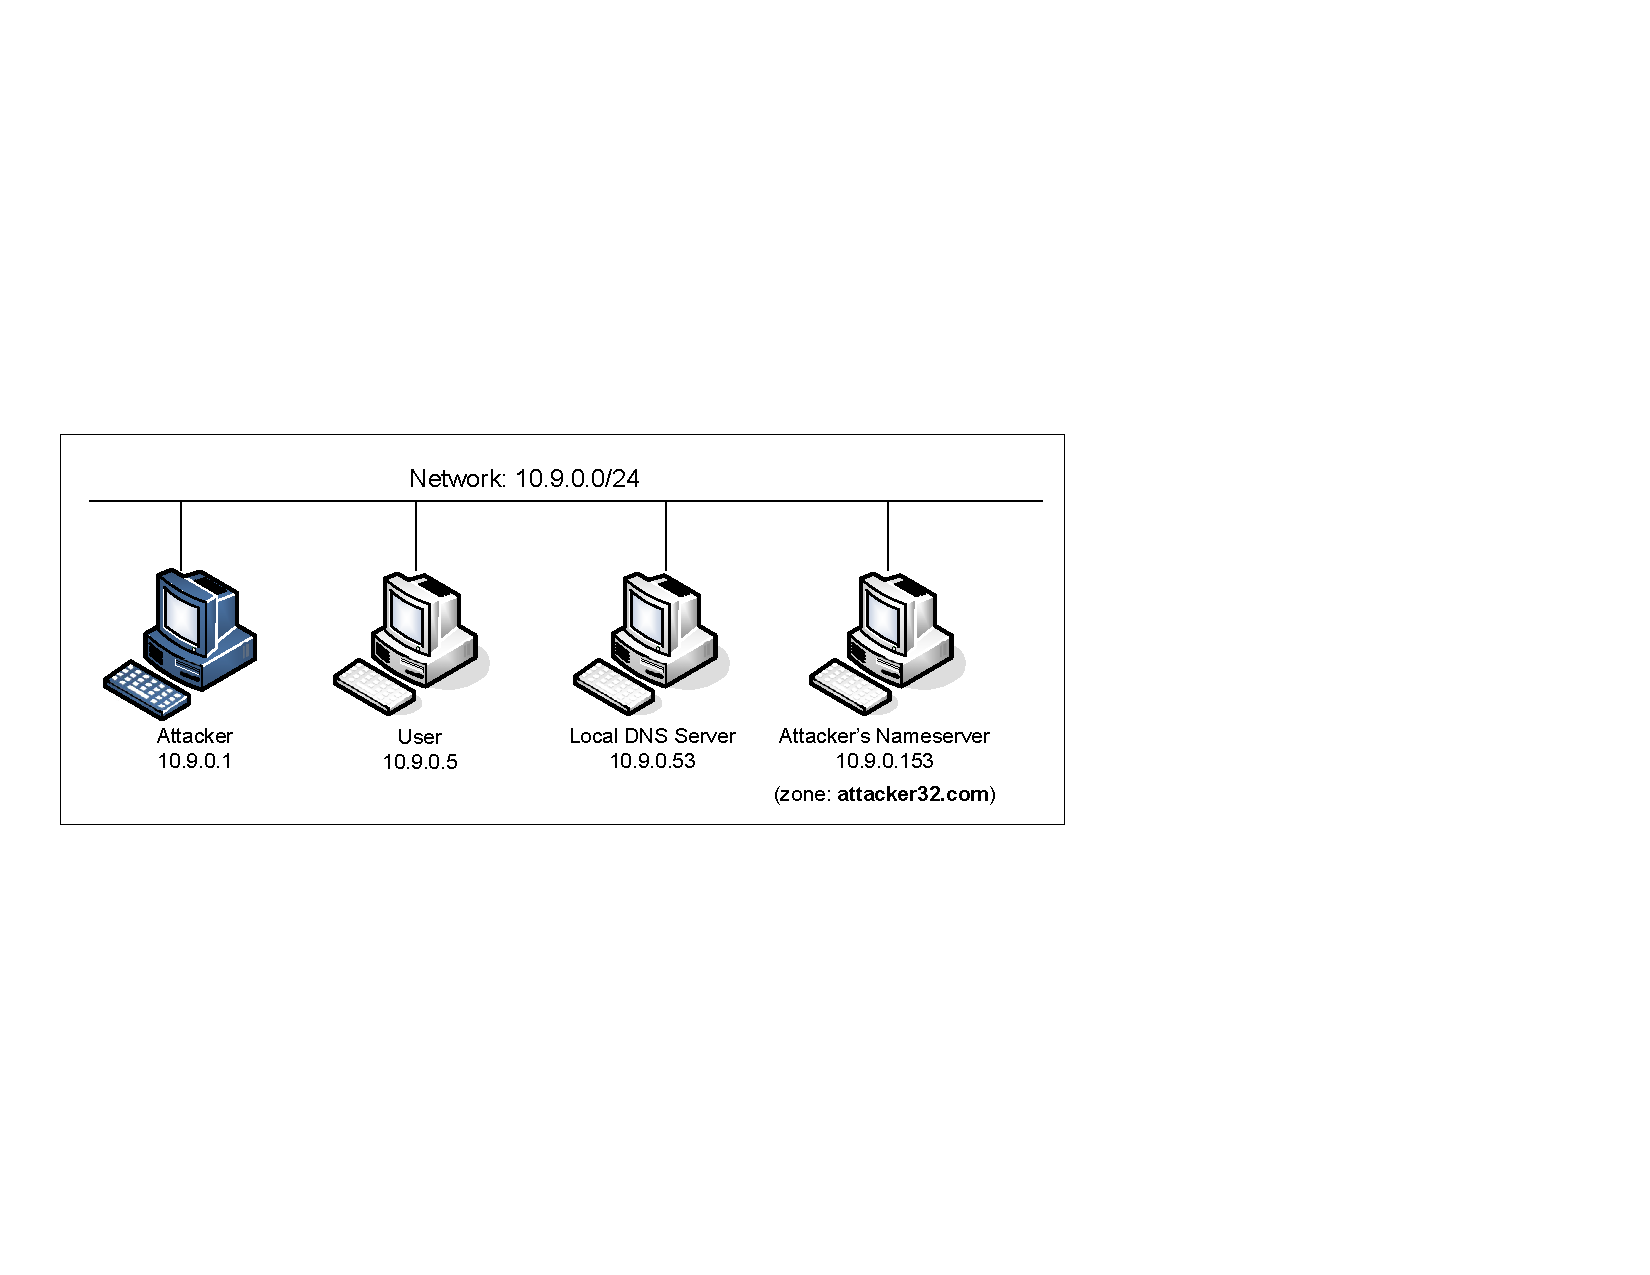
\includegraphics[width=0.85\textwidth]{\commonfolder/Figs/DNS.pdf}
\caption{Setup del Entorno}
\label{dns:fig:environment}
\end{figure}

El principal objetivo para un ataque de DNS cache poisoning es el servidor de DNS  local. Obviamente es ilegal atacar un servidor real, poor lo que necesitaremos crear y configurar nuestro propio servidor DNS para conducir los ataques en nuestros experimentos. El entorno de laboratorio necesita cuatro máquinas por separado:
una va a ser la máquina víctima, la segunda será el servidor de DNS local y las dos restantes serán las máquinas de los atacantes.
El setup del entorno del laboratorio se ilustra en la Figura \ref{dns:fig:environment}.


%\begin{lstlisting}[backgroundcolor=]
% +------------+   +------------+  +------------+  +---------------+
% | Attack VM  |   |  Container |  |  Container |  |  Container    |
% |            |   |   (user)   |  |  Local DNS |  |attacker32.com |
% |            |   |            |  |   Server   |  |  nameserver   |
% |  10.9.0.1  |   |  10.9.0.5  |  |  10.9.0.53 |  |  10.9.0.153   |
% +-----+------+   +------+-----+  +------+-----+  +------+--------+
%       |                 |               |               |
%       |                 |               |               |
%-------+-----------------+---------------+---------------+-------
%           Network  10.9.0.0/24
%
%\end{lstlisting}

Hemos puesto a todas las máquinas en la misma LAN con el objetivo de facilitar un poco todo.
Los estudiantes no pueden explotar este hecho en sus ataques; ellos deberían de considerar a la máquina del atacante como una máquina remota, es decir, el atacante no puede sniffear paquetes en la LAN.
Esto es diferente al ataque local del DNS.


% -------------------------------------------
% SUBSECTION
% -------------------------------------------
\subsection{Setup del Contenedor y sus Comandos}


%%%%%%%%%%%%%%%%%%%%%%%%%%%%%%%%%%%%%%%%%%%%
Para empezar a preparar el contenedor, deberá descargarse el archivo \texttt{Labsetup.zip} ubicado en el laboratorio correspondiente dentro del sitio web oficial y copiarlo dentro de la Máquina Virtual prevista por SEED. Una vez descargado deberá descomprimirlo y entrar dentro del directorio \texttt{Labsetup} donde encontrará el archivo \texttt{docker-compose.yml} que servirá para setear el entorno de laboratorio. Para una información más detallada sobre el archivo \texttt{Dockerfile} y otros archivos relacionados, puede encontrarla dentro del Manual de Usuario del laboratorio en uso, en el sitio web oficial de SEED.

Si esta es su primera experiencia haciendo el setup del laboratorio usando contenedores es recomendable que lea el manual anteriormente mencionado.

A continuación, se muestran los comandos más usados en Docker y Compose.
Debido a que estos comandos serán usados con mucha frecuencia, hemos creados un conjunto de alias para los mismos, ubicados en del archivo \texttt{.bashrc} dentro de la Máquina Virtual provista por SEED (Ubuntu 20.04)

\begin{lstlisting}
$ docker-compose build  # Build the container image
$ docker-compose up     # Start the container
$ docker-compose down   # Shut down the container

// Aliases for the Compose commands above
$ dcbuild       # Alias for: docker-compose build
$ dcup          # Alias for: docker-compose up
$ dcdown        # Alias for: docker-compose down
\end{lstlisting}


Dado que todos los contenedores estarán corriendo en un segundo plano. Necesitamos correr comandos para interactuar con los mismos, una de las operaciones fundamentales es obtener una shell en el contenedor. 
Para este propósito usaremos \texttt{"docker ps"} para encontrar el ID del contenedor deseado y ingresaremos \texttt{"docker exec"} para correr una shell en ese contenedor.
Hemos creado un alias para ello dentro del archivo \texttt{.bashrc}

\begin{lstlisting}
$ dockps        // Alias for: docker ps --format "{{.ID}}  {{.Names}}" 
$ docksh <id>   // Alias for: docker exec -it <id> /bin/bash

// The following example shows how to get a shell inside hostC
$ dockps
b1004832e275  hostA-10.9.0.5
0af4ea7a3e2e  hostB-10.9.0.6
9652715c8e0a  hostC-10.9.0.7

$ docksh 96
root@9652715c8e0a:/#  

// Note: If a docker command requires a container ID, you do not need to 
//       type the entire ID string. Typing the first few characters will 
//       be sufficient, as long as they are unique among all the containers. 
\end{lstlisting}

En caso de problemas configurando el entorno, por favor consulte la sección ``Common Problems'' en el manual ofrecido por SEED. 


%%%%%%%%%%%%%%%%%%%%%%%%%%%%%%%%%%%%%%%%%%%%



% -------------------------------------------
% SUBSECTION
% -------------------------------------------
\subsection{Sobre el Contenedor del Atacante}

Para este laboratorio podemos usar tanto una Máquina Virtual como un contenedor como máquina de ataque. Si observa el archivo Docker Compose, verá que el contenedor de ataque está configurado de forma diferente al resto de los contenedores.


\begin{itemize}
\item \textit{Directorio Compartido.} Cuando usemos el contenedor del atacante para realizar los ataques, necesitamos poner el código de ataque dentro del contenedor.
%%%%%%%%%%%%%%%%%%%%%%%%%%%%%%%%%%%%%%%%%%%%%%%
Code editing is more convenient inside the VM than in containers, 
because we can use our favorite editors.
In order for the VM and container to share files, 
we have created a shared folder between the VM and the container
using the Docker \texttt{volumes}.
If you look at the Docker Compose file, you will find out that
we have added the following entry to some of the containers.
It indicates mounting the \texttt{./volumes} folder on the host
machine (i.e., the VM) to the \texttt{/volumes} folder inside the container.
We will write our code in the \texttt{./volumes} folder (on the VM), so they
can be used inside the containers.

\begin{lstlisting}
volumes:
       - ./volumes:/volumes
\end{lstlisting}


%%%%%%%%%%%%%%%%%%%%%%%%%%%%%%%%%%%%%%%%%%%%%%%


\item \textit{Host mode.}
%%%%%%%%%%%%%%%%%%%%%%%%%%%%%%%%%%%%%%%%%%%%%%%
In this lab, the attacker needs to be able to sniff packets,
but running sniffer programs inside a container has problems, because
a container is effectively attached to a virtual switch, 
so it can only see its own traffic, and it is never going to see 
the packets among other containers. To solve this problem,
we use the \texttt{host} mode for the attacker container. This
allows the attacker container to see all the traffics. The following
entry used on the attacker container:

\begin{lstlisting}
network_mode: host
\end{lstlisting}

When a container is in the \texttt{host} mode,  it sees
all the host's network interfaces, and it even has the same
IP addresses as the host. Basically, it is put in the
same network namespace as the host VM. However, the container
is still a separate machine, because its other namespaces are
still different from the host.


%%%%%%%%%%%%%%%%%%%%%%%%%%%%%%%%%%%%%%%%%%%%%%%
\end{itemize}





% -------------------------------------------
% SUBSECTION
% -------------------------------------------
%%%%%%%%%%%%%%%%%%%%%%%%%%%%%%%%%%%%%%%%%%%%
%%%%%%%%%%%%%%%%%%%%%%%%%%%%%%%%%%%%%%%%%%%%%%%%%%%%%%%%%%%%%%%%%%%%%%
%%  Copyright by Wenliang Du.                                       %%
%%  This work is licensed under the Creative Commons                %%
%%  Attribution-NonCommercial-ShareAlike 4.0 International License. %%
%%  To view a copy of this license, visit                           %%
%%  http://creativecommons.org/licenses/by-nc-sa/4.0/.              %%
%%%%%%%%%%%%%%%%%%%%%%%%%%%%%%%%%%%%%%%%%%%%%%%%%%%%%%%%%%%%%%%%%%%%%%


% -------------------------------------------
% SUBSECTION
% ------------------------------------------- 
\subsection{Resumen de la Configuración del DNS} 

Todos los contenedores han sido configurados para este laboratorio.
Por lo que haremos un resumen de ellos, de esta manera los estudiantes estarán al tanto de estas configuraciones. Para explicaciones más detalladas sobre las configuraciones puede consultar el manual.



\paragraph{Servidor de DNS local.} 
Como servidor de DNS local usaremos el software BIND 9.
BIND 9 carga su configuración de un archivo llamado \path{/etc/bind/named.conf}. Este es el principal archivo de configuración y usualmente contiene varias entradas de \texttt{"include"}, por medio de este include puede cargar las configuraciones de diferentes archivos. Uno de los archivos usado por ese include es llamado \path{/etc/bind/named.conf.options}. Es en este archivo donde se establece la configuración actual.


\begin{itemize}
\item \textit{Simplificación.}
Los servidores DNS hoy en día randomizan el número de puerto de origen en sus consultas DNS; esto hace que los ataques sean mucho más difíciles. Desafortunadamente, muchos servidores DNS siguen usando número de puertos de origen predecibles. Para simplificar este laboratorio, hemos fijado el número de puerto de origen a {\tt 33333} dentro del archivo de configuración.

\item \textit{Desactivando DNSSEC.} 
DNSSEC fue introducido como mecanismo de protección en contra de ataques de spoofing en los servidores DNS. Para mostrar como funciona este ataque, hemos desactivado esta protección en el archivo de configuración.

\item \textit{DNS caché.}
Durante el ataque, necesitaremos inspeccionar la caché DNS en el servidor de DNS local. Los siguientes dos comando sirven para este propósito.
El primer comando hace un dump del contenido de la caché en el archivo \path{/var/cache/bind/dump.db}, y el segundo comando limpia la caché.

\begin{lstlisting}
# rndc dumpdb -cache    // Dump the cache to the specified file
# rndc flush            // Flush the DNS cache
\end{lstlisting}

\item \textit{Forwardeo de la zona \texttt{attacker32.com}.}
Una zona de forwardeo es agregada en el servidor de DNS local, por lo que si alguien quiere consultar el dominio \texttt{attacker32.com}, la consulta será forwardeada al nameserver de este dominio, que será hosteado en el contenedor del atacante. La entrada para esta zona se ubcica dentro del archivo \texttt{named.conf}.

\begin{lstlisting}
zone "attacker32.com" {
    type forward;
    forwarders { 
        10.9.0.153; 
    };
};
\end{lstlisting}
\end{itemize}



\paragraph{Máquina del Usuario.}
El contenedor del usuario cuya dirección IP es {\tt 10.9.0.5} está configurada para usar la dirección IP {\tt 10.9.0.53} como su servidor DNS local.
Esto se logra cambiando la configuración del archivo de resolución de la máquina del usuario (\texttt{/etc/resolv.conf}), se agrega el servidor \texttt{10.9.0.53}  como \texttt{nameserver} en la primera línea del archivo, de esta forma la máquina entenderá que este será el servidor DNS primario usado por defecto.


\paragraph{Nameserver del Atacante.}
Dentro de la máquina del atacante, se hostean dos zonas. La primera es la zona legítima del atacante \texttt{attacker32.com}, y la segunda es la zona falsa del dominio \texttt{example.com}. Las zonas son configuradas en el archivo \path{/etc/bind/named.conf}:

\begin{lstlisting}
zone "attacker32.com" {
        type master;
        file "/etc/bind/attacker32.com.zone";
};

zone "example.com" {
        type master;
        file "/etc/bind/example.com.zone";
};
\end{lstlisting}


%%%%%%%%%%%%%%%%%%%%%%%%%%%%%%%%%%%%%%%%%%%%%%%%%%%%%%%%%%%%%%%%%%%%%%
%%  Copyright by Wenliang Du.                                       %%
%%  This work is licensed under the Creative Commons                %%
%%  Attribution-NonCommercial-ShareAlike 4.0 International License. %%
%%  To view a copy of this license, visit                           %%
%%  http://creativecommons.org/licenses/by-nc-sa/4.0/.              %%
%%%%%%%%%%%%%%%%%%%%%%%%%%%%%%%%%%%%%%%%%%%%%%%%%%%%%%%%%%%%%%%%%%%%%%


% -------------------------------------------
% SUBSECTION
% ------------------------------------------- 
\subsection{Testing the DNS Setup}

From the User container, we will run a series of commands to ensure 
that our lab setup is correct. In your lab report, please document
your testing results. 


\paragraph{Get the IP address of \texttt{ns.attacker32.com}.}
When we run the following \texttt{dig} command, 
the local DNS server will forward the request to the Attacker nameserver 
due to the \texttt{forward} zone entry added to the local DNS server's
configuration file. Therefore, the answer should come from
the zone file (\texttt{attacker32.com.zone}) that we set up on the Attacker nameserver.
If this is not what you get, your setup has issues. Please describe your
observation in your lab report. 

\begin{lstlisting}
$ dig ns.attacker32.com
\end{lstlisting}



\paragraph{Get the IP address of \texttt{www.example.com}.} 
Two nameservers are now hosting the \texttt{example.com} 
domain, one is the domain's official nameserver, and the other 
is the Attacker container. We will query these two nameservers and see what 
response we will get. 
Please run the following two commands (from the User machine), 
and describe your observation. 


\begin{lstlisting}
// Send the query to our local DNS server, which will send the query
// to example.com's official nameserver. 
$ dig www.example.com

// Send the query directly to ns.attacker32.com 
$ dig @ns.attacker32.com www.example.com
\end{lstlisting}
 


Obviously, nobody is going to ask \texttt{ns.attacker32.com} for 
the IP address of \texttt{www.example.com}; they will always ask
the \texttt{example.com} domain's official nameserver for 
answers. The objective of the DNS cache poisoning attack
is to get the victims to ask 
\texttt{ns.attacker32.com} for the IP address of 
\texttt{www.example.com}. Namely, if our attack is successful, 
if we just run the first \texttt{dig} command, the one
without the \texttt{@} option, we should get the 
fake result from the attacker, instead of getting 
the authentic one from the domain's legitimate nameserver.



%%%%%%%%%%%%%%%%%%%%%%%%%%%%%%%%%%%%%%%%%%%%



% *******************************************
% SECTION
% ******************************************* 
\section{Las tareas de ataque}

El principal objetivo de los ataques DNS sobre un usuario es poder redireccionar al usuario hacia una máquina $B$ cuando el usuario intente acceder a una máquina $A$ usando el hostname de $A$. Por ejemplo, cuando un usuario trata de acceder al online banking, los atacantes pueden redireccionarlo a un sitio web malicioso que luce casi igual al sitio oficial del banco, en consecuencia el usuario puede ser engañado y así los atacantes pueden obtener sus credenciales bancarias.

En esta tarea, vamos a usar el nombre de dominio {\tt www.example.com} como nuestro objetivo para hacer el ataque. Cabe señalar que el dominio {\tt www.example.com} está reservado solamente para el uso experimental dentro del contexto de este laboratorio y no para el mundo real. La dirección IP real de {\tt www.example.com} es {\tt 93.184.216.34} y su nameserver es controlado por la Internet Corporation for Assigned Names and Numbers (ICANN).
Cuando el usuario ejecuta el comando {\tt dig} sobre este dominio o usa el navegador para visitarlo, la máquina del usuario envia una consulta DNS a su servidor de DNS local que consultará la dirección IP usando el nameserver de {\tt example.com}.

La meta del ataque es ejecutar un ataque de DNS cache poisoning attack en el servidor de DNS local, de tal forma que cuando el usuario ejecute el comando {\tt dig} para obtener la dirección IP de {\tt www.example.com}, el servidor de DNS local terminará consultando el nameserver del atacante {\tt ns.attacker32.com} y así obtendrá la dirección IP definida por atacante. Como resultado final el usuario será dirigido al sitio web del atacante en lugar del sitio original {\tt www.example.com}.



\begin{figure}[htb]
\centering
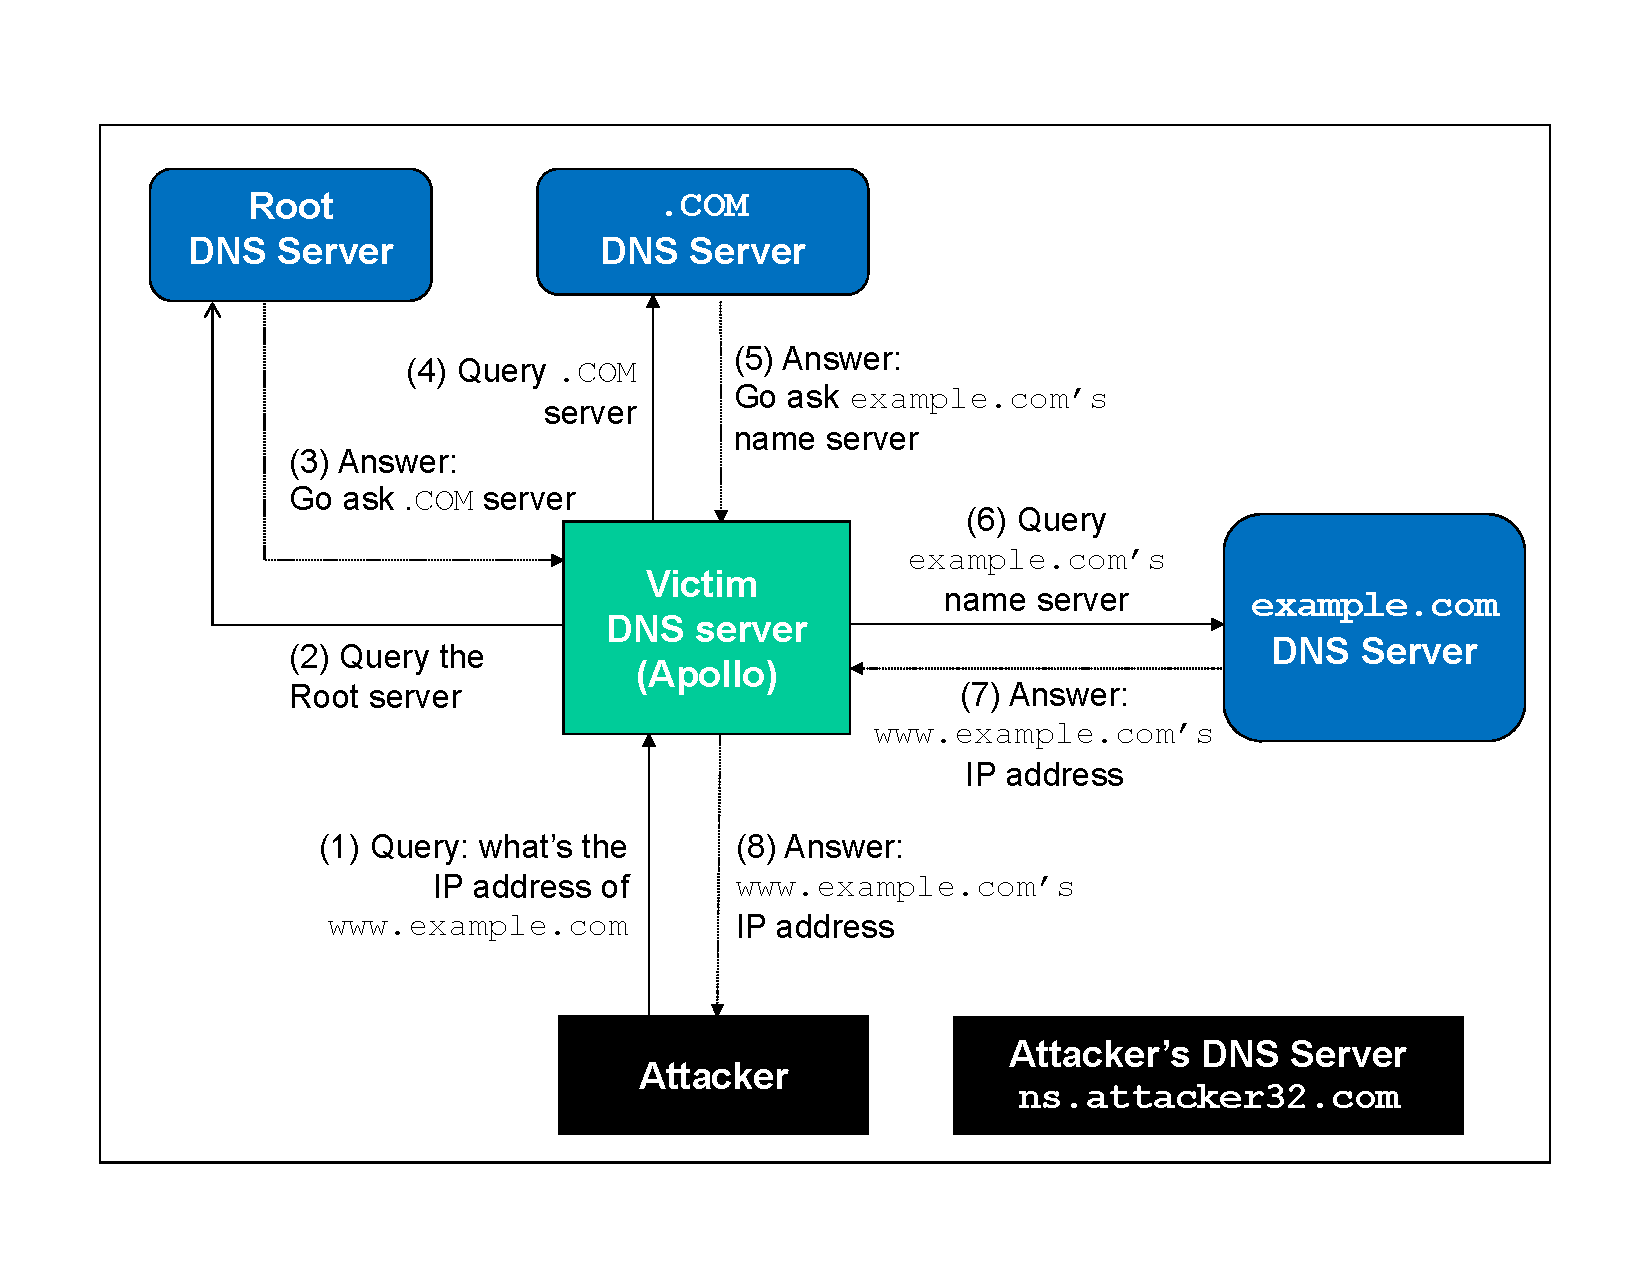
\includegraphics[width=0.9\textwidth]{\dnsFigs/DNS_Remote_new1.pdf}
\caption{El proceso de consulta DNS} 
\label{fig:flow_diagram1}
\end{figure}


\begin{figure}[htb]
\centering
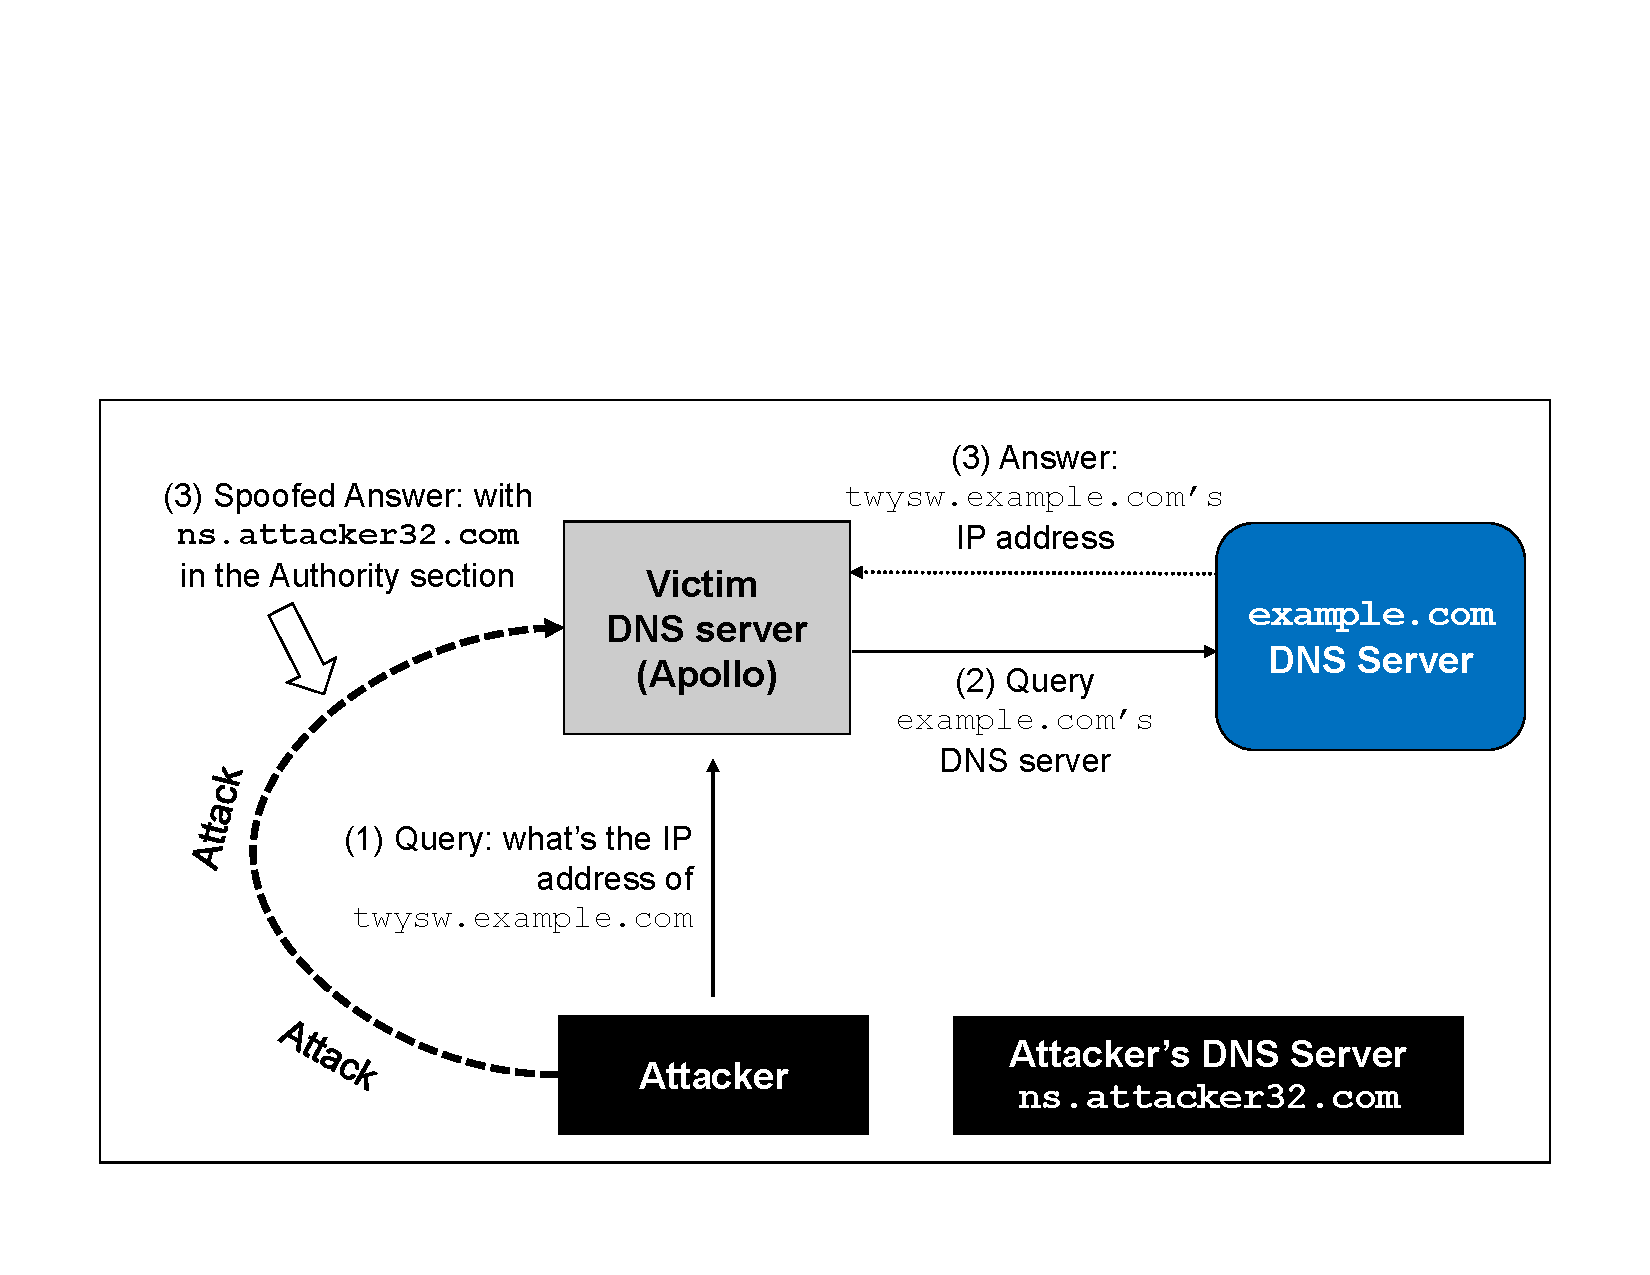
\includegraphics[width=0.9\textwidth]{\dnsFigs/DNS_Remote_new2.pdf}
\caption{El Ataque Kaminsky}
\label{fig:flow_diagram2}
\end{figure}



% -------------------------------------------
% SUBSECTION
% ------------------------------------------- 
\subsection{Como funciona el Ataque de Kaminsky}

En esta tarea, el atacante envía una consulta de petición DNS al servidor DNS de la víctima ({\tt Apollo}), activando una consulta DNS desde {\tt Apollo}.
La consulta puede viajar a través de uno de los servidores DNS raíz, el servidor DNS {\tt .COM} y el resultado final vendrá desde el servidor DNS de {\tt example.com}. Esto se ilustra en la Figura \ref{fig:flow_diagram1}. En caso que la información del nameserver para el dominio {\tt example.com} esté cacheada por {\tt Apollo}, la consulta no irá al servidor raíz o al servidor {\tt .COM}; esto se ilustra en la Figura \ref{fig:flow_diagram2}.
En este laboratorio, la situación representadda en la Figura \ref{fig:flow_diagram2} es la más común, por lo que usaremos esta figura como base para describir el mecanismo de ataque.

Mientras {\tt Apollo} espera por la respuesta DNS del nameserver de  {\tt example.com}, el atacante puede enviar respuestas falsificadas/spoofeadas a {\tt Apollo}, fingiendo que las respuesta provienen del nameserver de {\tt example.com}. Si la respuesta falsificada llega primero, será aceptada por {\tt Apollo}. Podemos decir que el ataque fue exitoso.

Si ud. ha hecho el laboratorio de Ataque de DNS local, debería de saber que esos ataques asumen que el atacante y el servidor DNS están en la misma LAN, es decir el atacante puede observar el mensaje de una consulta DNS.
Cuando el atacante y el servidor DNS no se encuentran en la misma LAN, el ataque de cache poisoning se vuelve un poco más difícil.
La dificultad es causada por el hecho que el ID de transacción en el paquete de respuesta DNS debe de coincidir con el del paquete de la consulta. Dado que el ID de transacción en la consulta es generado de forma aleatoria, sin poder observar el paquete de consulta, no es fácil para un atacante saber el ID correcto.

Obviamente, el atacante puede adivinar el ID de transacción, dado que el tamaño de este ID es de sólo 16 bits, si el atacante puede falsificar/spoofear $K$ respuestas dentro de la ventana de ataque (es decir antes que la respuesta legítima llegue a destino), la probabilidad de suceso de $K$ es de $2^{16}$. 
Enviar cientos de respuestas falsas no es poco práctico, por lo que
no serán necesarios muchos intentos antes de que el atacante pueda tener éxito.

Sin embargo, el hipotético ataque que se planteó anteriormente ha pasado por alto el efecto de la caché.
En realidad, si el atacante no es lo suficientemente afortunado en su trabajo de adivinar el ID correcto antes de que el paquete de la respuesta original llegue a su destino, la información correcta será cacheada por un período de tiempoo en el servidor DNS. Este efecto de almacenamiento en la caché, hace imposible que el atacante pueda falsificar otra respuesta con respecto al mismo nombre, dado que el servidor DNS no enviará otra consulta DNS para este nombre hasta que expiré la caché para este nombre.
Para falsificar la respuesta sobre el mismo nombre, el atacante tiene que esperar por otra consulta DNS sobre este nombre, lo que significa que debe de esperar que la caché expire. El tiempo de expiración puede estar en el orden de la horas o de los días.


\paragraph{El Ataque de Kaminsky.} 
Dan Kaminsky ideó una técnica para evadir este efecto del almacenamiento en la caché \cite{dns:Kaminsky}.
Con el ataque de Kaminsky, los atacantes tienen la posibilidad de atacar continuamente un servidor DNS en un nombre de dominio específico sin la necesidad de esperar que la caché expire, por lo que los ataques pueden ser exitosos en un tiempo relativamente corto. 
Los detalles del ataque son descriptos en \cite{dns:Kaminsky,seedbook}. 
En esta tarea, usaremos este ataque. Los siguientes pasos que hacen referencia a la Figura \ref{fig:flow_diagram2} que describe el ataque.


\begin{enumerate}

\item El atacante consulta el servidor DNS {\tt Apollo} por un nombre no existente en {\tt example.com} por ejemplo {\tt twysw.example.com}, donde {\tt twysw} es un nombre aleatorio.
 
\item Dado que este mapeo no está disponible en la cache del DNS de {\tt Apollo},
{\tt Apollo} envía una consulta DNS al nameserver del dominio  {\tt example.com}.

\item Mientras que {\tt Apollo} espera por la respuesta, el atacante  inunda {\tt Apollo} con un flujo de respuesta DNS falsificadas, en cada una de estas respuestas se prueba un ID de transacción diferente esperando que alguna sea correcta.
En la respuesta, el atacante no solo proporciona una resolución de IP
para {\tttwysw.example.com}, el atacante también proporciona un registro de ``Authoritative Nameservers'', indicando a {\tt ns.attacker32.com} como nameserver para el dominio {\tt example.com}.
Si la respuesta falsificada supera a las respuestas reales y el ID de transacción coincide con el de la consulta, {\tt Apollo} va a aceptarla y cacheará la respuesta falsificada por lo que la caché DNS de {\tt Apollo} está envenenada (poisoned)

\item Incluso si la respuesta DNS que se falsificó/spoofeo falla (por ejemplo el ID de transacción no coincide o llega tarde), no importa, porque la próxima vez, el atacante consultará un nombre diferente, por lo que {\tt Apollo} deberá de enviar otra consulta dándole al atacante otra chance de hacer un ataque de este tipo.
Definitivamente este ataque evade el efecto del almacenamiento en la caché.

\item Si el ataque funciona, en la caché DNS de {\tt Apollo}, el nameserver para {\tt example.com} será reemplazado con el que proporciona el atacante {\tt ns.attacker32.com}.
Para demostrar que el ataque funciona, los estudiantes deben de mostrar que tal registro se encuentra dentro de la caché DNS de {\tt Apollo}.

\end{enumerate}


\paragraph{Descripción de la Tarea.} La implementación del ataque de Kaminsky es algo desafiante, por lo que la hemos separado en varias sub-tareas.
En la Tarea 2, construíremos petición DNS para un hostname aleatorio usando el dominio \texttt{example.com}. En la Tarea 3, construíremos spoofearemos las respuestas provenientes del nameserver en \texttt{example.com}. En la Tarea 4, pondremos todo junto para lanzar el ataque de Kaminsky y finalmente en la Tarea 5, verificaremos el impacto del ataque.

% -------------------------------------------
% SUBSECTION
% ------------------------------------------- 
\subsection{Tarea 2: Construyendo una petición DNS} 

Esta tarea se centra en el envío de peticiones DNS.
Para completar el ataque, los atacantes necesitan hacer que el servidor DNS envié consultas, de esta forma tendrán las chances necesarias para empezar a falsificar respuestas DNS. Dado que los atacantes necesitan intentar varias veces antes de que el ataque sea exitoso, es mejor automatizar el proceso usando un programa.

Los estudiantes deben escribir un programa para enviar consultas DNS al servidor DNS objetivo (es decir, el servidor de DNS local de nuestro setup).
La tarea de los estudiantes es escribir este programa y demostrar (usando Wireshark) que sus consultas hacen que el servidor DNS objetivo esté enviando las consultas DNS correspondientes.
Los requerimientos de performance para esta tarea no son altos, por lo que lo estudiantes pueden usar C o Python (con Scapy) para desarrollar el código del programa.
A continuación se muestra un fragmento de código (los \texttt{+++} son placeholders; los estudiantes deben de reemplazarlos con los valores pertinentes):


\begin{lstlisting}
Qdsec  = DNSQR(qname='www.example.com')
dns    = DNS(id=0xAAAA, qr=0, qdcount=1, ancount=0, nscount=0,
             arcount=0, qd=Qdsec)

ip  = IP(dst='+++', src='+++')
udp = UDP(dport=+++, sport=+++, chksum=0)
request = ip/udp/dns
\end{lstlisting}
 


% -------------------------------------------
% SUBSECTION
% ------------------------------------------- 
\subsection{Tarea 3: Spoofeando respuestas DNS.}   

En esta tarea, necesitamos spoofear las respuestas DNS en el ataque de Kaminsky.
Dado que nuestro objetivo es  \texttt{example.com}, necesitamos spoofear las respuesta del nameserver para este dominio. Los estudiantes primero necesitarán descubrir la dirección IP de los nameservers originales de  \texttt{example.com} (cabe señalar que existen multiples nameservers para este dominio).

Los estudiantes pueden usar Scapy para implementar esta tarea. El siguiente fragmento de código, construye un paquete que representa una respuesta DNS que incluye la sección Question, una sección Answer y una sección NS.
En este código deejemplo, usarmos \texttt{+++} como placeholders; los estudiantes deben de reemplazar estos placeholders con los valores correctos que son necesarios para el ataqu de Kaminsky. Los estudiantes deben de explicar porque escogieron esos valores.


\begin{lstlisting}
name   = '+++'  
domain = '+++'  
ns     = '+++'

Qdsec  = DNSQR(qname=name)
Anssec = DNSRR(rrname=name,   type='A',  rdata='1.2.3.4', ttl=259200)
NSsec  = DNSRR(rrname=domain, type='NS', rdata=ns, ttl=259200)
dns    = DNS(id=0xAAAA, aa=1, rd=1, qr=1,
             qdcount=1, ancount=1, nscount=1, arcount=0,
             qd=Qdsec, an=Anssec, ns=NSsec)

ip    = IP(dst='+++', src='+++')
udp   = UDP(dport=+++, sport=+++, chksum=0)
reply = ip/udp/dns
\end{lstlisting}
 
Dado que esta respuesta por sí sóla no será capaz de conducir a un ataque exitoso, para demostrar lo hecho en esta tarea, los estudiantes deberán de usar Wireshark para capturar las respuestas DNS spoofeadas y mostrar que los paquetes spoofeados son válidos.


% -------------------------------------------
% SUBSECTION
% ------------------------------------------- 
\subsection{Tarea 4: Lanzar el Ataque de Kaminsky}   

Ahora que hemos puesto todo junto, estamos listos para realizar el ataque de Kaminsky.
En este ataque, necesitamos enviar muchas respuestas DNS spoofeadas, con la esperanza de que alguna de ellas entre en el número correcto de transacción y llegue antes que la respuesta original.
La velocidad es esencial en este asunto: mientras más paquetes enviemos, más posibilidades tendremos de que el ataque sea exitoso.
Si usamos Scapy para enviar respuestas DNS spoofeadas como hicimos en las tareas anteriores, la taza de exito será baja. Los estudiantes pueden usar C, pero construir paquetes DNS en C es algo no trivial.
Vamos a introducir un enfoque híbrido usando Scapy y C (vea el libro de SEED para más detalles)

Con este enfoque híbrido, primero usaremos Scapy para generar un paquete DNS que sirva como planilla, esta será guardada en un archivo.
Luego, cargaremos esta planilla dentro de un programa en C, y le haremos unos pequeños cambios a algunos de sus campos y por último enviaremos este paquete.
Hemos incluído un código base en C dentro de  \path{Labsetup/Files/attack.c}. 
Los estudiantes pueden realizar cambios en las áreas que están marcadas. Para una explicación mas detallada consulte la sección Guías.



\paragraph{Chequear la caché DNS.}
Para chequear si el ataque fue exitoso o no, necesitamos chequear el archivo  {\tt dump.db} para ver si nuestra respuesta DNS spoofeada fue aceptada por el servidor DNS.
El siguiente comando hace un dump de la caché DNS y se encarga de buscar si la palabra \texttt{attacker} se encuentra dentro de la caché (en nuestro ataque hemos usado \texttt{attacker32.com} como el dominio del atacante, si los estudiantes desean usar un nombre diferente, deberían de buscar por una palabra difernte)

\begin{lstlisting}
# rndc dumpdb -cache && grep attacker /var/cache/bind/dump.db
\end{lstlisting}
 

% -------------------------------------------
% SUBSECTION
% ------------------------------------------- 
\subsection{Tarea 5: Verificación del Resultado}

Si el ataque es exitoso, veremos en la caché del servidor de DNS local, el registro {\tt NS} para \texttt{example.com} será \texttt{ns.attacker32.com}.
Cuando este servidor recibe una consulta DNS para cualquier hostname dentro del dominio \texttt{example.com}, este enviará una consulta a \texttt{ns.attacker32.com}, en lugar de enviarla al nameserver original del dominio.

Para verificar si el ataque fue exitoso o no, vaya a la máquina de usuario y corra los siguientes dos comandos usando \texttt{dig}. En las respuesta, la direcciones IP para \texttt{www.example.com} deberían de ser las mismas para ambos comandos, y debería de ser lo que haya incluído en el archivo de la zona del nameserver del atacante.

\begin{lstlisting}
// Ask the local DNS server to do the query
$ dig www.example.com

// Directly query the attacker32 nameserver
$ dig @ns.attacker32.com www.example.com
\end{lstlisting}
 
Por favor incluya su observación (capturas de pantalla) en el informe del laboratorio y explique porque ud. piensa que su ataque fue exitoso.
En particular, cuando corra el primer comando \texttt{dig} use Wireshark para capturar el tráfico de red y señalar que paquetes son disparados por este comando  \texttt{dig}. Use el trackeo del paquete para probar que su ataque es exitoso. Note que los resultados en el servidor de DNS local pueden estar cacheados después de que correr por primera vez el comando \texttt{dig}. Esto puede influenciar en los resultados si ud. corre el comando \texttt{dig} antes de usar Wireshark. Puede limpiar la caché usando  \texttt{"sudo rndc flush"}  en el servidor de DNS local, pero esto requerirá que ud. lance nuevamente el ataque.


% *******************************************
% SECTION
% ******************************************* 
\section{Guías} 

Para implementar el ataque de Kaminsky, podemos usar Scapy para hacer spoofing de paquetes. Desafortunadamente la velocidad de Python es demasiado lenta; el número de paquetes generados por segundo son insuficientes para que el ataque tenga éxito. Es mejor usa un programa hecho en C. Esto puede ser algo desafiante para mucho de los estudiantes, porque construir un paquete DNS usando C no es tan fácil.
He desarrollado un método híbrido y lo hemos usado en mis clases. Usando este enfoque, el tiempo que tardan los estudiantes en desarrollar el programa se ve reducido de manera significativa, esto es beneficioso ya que pueden concentrarse mucho más tiempo en el ataque en sí.

La idea es unir las fuerzas de Scapy y C: Scapy es mucho mas conveniente en la creación de paquetes DNS que C. Hemos usado Scapy para crear paquetes DNS spoofeados y guardarlos en un archivo, para después cargar estos paquetes dentro de un programa en C. Aunque necesitamos enviar mucho paquetes DNs durante el ataque de Kaminsky, esos paquetes son bastantes similares, exepto por algunos pocos campos.
Podemos usar a Scapy para generar paquetes que sirvan como base para encontrar los offsets en donde esos cambios deben de realizarse (Ejemplo: el campo de ID de Transacción) y hacer directamente el cambio sobre el. Esto será mucho más fácil que crear el paquete DNS en C.
Despues de que los cambios se han realizado podemos usar raw sockets para enviar esos paquetes.
Los detalles de este método híbrido son provistos en el capítulo de Packet Sniffing and Spoofing en el libro de SEED \cite{seedbook}.
El siguiente programa usa Scapy para crear un paquete de respuesta DNs bastante simple y lo guarda en un archivo.

\begin{lstlisting}[caption={\texttt{generate\_dns\_reply.py}}]
#!/usr/bin/env python3
from scapy.all import *

# Construct the DNS header and payload
name   = 'twysw.example.com'
Qdsec  = DNSQR(qname=name)
Anssec = DNSRR(rrname=name, type='A', rdata='1.1.2.2', ttl=259200)
dns    = DNS(id=0xAAAA, aa=1, rd=0, qr=1, 
             qdcount=1, ancount=1, nscount=0, arcount=0, 
             qd=Qdsec, an=Anssec)

# Construct the IP, UDP headers, and the entire packet
ip  = IP(dst='10.0.2.7', src='1.2.3.4', chksum=0)
udp = UDP(dport=33333, sport=53, chksum=0)
pkt = ip/udp/dns

# Save the packet to a file
with open('ip.bin', 'wb') as f:
  f.write(bytes(pkt))
\end{lstlisting}

En el programa en C, cargamos este paquete desde un archivo llamado  \texttt{ip.bin} y lo usamos como nuestro paquete planilla (template), a partir del mismo crearemos varios paquetes similares y haremos un flood con estos paquetes spoofeados de respuesta al servidor de DNS local.
Por cada respuesta, debemos de cambiar tres lugares: el ID de transacción y el nombre \texttt{twysw} que aparece en dos lugares (la sección Question y la sección Answer). El ID de transacción siempre se encuentra en el mismo lugar (offset \texttt{28} a partir del comienzo de nuestro paquete IP), pero el offset para el nombre \texttt{twysw} depende de la longitud del nombre de dominio. Podemos usar un editor binario como \texttt{bless} para visualizar el archivo binario \texttt{ip.bin} y encontrar los dos offsets donde se encuentra la cadena \texttt{twysw}. En nuestro paquete se encuentran en los offsets \texttt{41} y \texttt{64}.

El siguiente fragmento de código muestra hacer los cambios en esos campos. Cambiamos el nombre en nuestra respuesta a \texttt{bbbbb.example.com} y enviamos una respuesta DNS spoofeada con el ID de transacción que es \texttt{1000}. En este código la variable  \texttt{ip} apunta al comienzo del paquete IP.

\begin{lstlisting}
  // Modify the name in the question field (offset=41)
  memcpy(ip+41, "bbbbb" , 5);

  // Modify the name in the answer field (offset=64)
  memcpy(ip+64, "bbbbb" , 5);

  // Modify the transaction ID field (offset=28)
  unsigned short id = 1000;
  unsigned short id_net_order = htons(id);
  memcpy(ip+28, &id_net_order, 2);
\end{lstlisting}



\paragraph{Generar Nombres Aleatorios.} En el ataque de Kaminsky, necesitamos generar nombres aleatorios. Hay muchas formas de hacerlo. El siguiente fragmento de código muestra como generar un nombre aleatorio de 5 caracteres.
\begin{lstlisting}
char a[26]="abcdefghijklmnopqrstuvwxyz";

// Generate a random name of length 5
char name[6];
name[5] = 0;
for (int k=0; k<5; k++)  
   name[k] = a[rand() % 26];
\end{lstlisting}
 



% *******************************************
% SECTION
% ******************************************* 
\section{Informe del Laboratorio}

%%%%%%%%%%%%%%%%%%%%%%%%%%%%%%%%%%%%%%%%

Debe enviar un informe de laboratorio detallado, con capturas de pantalla, para describir lo que ha hecho y lo que ha observado.
También debe proporcionar una explicación a las observaciones que sean interesantes o sorprendentes.
Enumere también los fragmentos de código más importantes seguidos de una explicación. No recibirán créditos aquellos fragmentos de códigos que no sean explicados.
%%%%%%%%%%%%%%%%%%%%%%%%%%%%%%%%%%%%%%%%


% *******************************************
% SECTION
% *******************************************
\section*{Agradecimientos}

Este documento ha sido traducido al Español por Facundo Fontana



%%%%%%%%%%%%%%%%%%%%%%%%%%%%%%%%%%%%%%%%%%
\thispagestyle{empty}
\bibliographystyle{plain}
\def\baselinestretch{1}
\bibliography{BibDNS}
%%%%%%%%%%%%%%%%%%%%%%%%%%%%%%%%%%%%%%%%%%



\end{document}




